\documentclass[11pt]{article}

% ---------- Page ----------
\usepackage[a4paper,margin=24mm,top=22mm,bottom=24mm]{geometry}
\usepackage[T1]{fontenc}
\usepackage[utf8]{inputenc}

% ---------- Fonts ----------
\usepackage{XCharter}
\usepackage[scaled=0.95]{sourcesanspro}
\usepackage[bigdelims]{newtxmath}
\usepackage{microtype}

% ---------- Layout helpers ----------
\usepackage{xcolor}
% ---- Shared palette + TikZ styles (used by the doc and the standalone diagram) ----
\usepackage{tikz}
\usetikzlibrary{arrows.meta,positioning,fit,backgrounds,calc,shapes.geometric,shadows.blur}

\definecolor{ink}{HTML}{1E293B}
\definecolor{subink}{HTML}{475569}
\definecolor{accent}{HTML}{4338CA}   % indigo
\definecolor{teal}{HTML}{0F766E}
\definecolor{amber}{HTML}{B45309}
\definecolor{rose}{HTML}{9F1239}
\definecolor{slate}{HTML}{64748B}
\definecolor{mist}{HTML}{F1F5F9}
\definecolor{mist2}{HTML}{E9EEF5}
\definecolor{line}{HTML}{C7D2DE}

\tikzset{
  font=\sffamily\small,
  >={Stealth[round]},
  base/.style={
    rounded corners=3pt, draw=line, line width=0.7pt, fill=white,
    text=ink, align=center, inner sep=6pt, minimum height=9mm,
    minimum width=24mm
  },
  accentbox/.style={base, draw=accent, fill=accent!7, text=ink},
  tealbox/.style={base, draw=teal, fill=teal!8, text=ink},
  amberbox/.style={base, draw=amber, fill=amber!8, text=ink},
  store/.style={
    cylinder, shape border rotate=90, aspect=0.28, draw=slate,
    line width=0.7pt, fill=mist, text=ink, align=center,
    inner sep=5pt, minimum height=11mm, minimum width=22mm, font=\sffamily\small
  },
  ext/.style={base, draw=slate, fill=mist, text=subink, minimum width=20mm},
  group/.style={rounded corners=6pt, draw=line, line width=0.7pt, fill=mist!55},
  grouplabel/.style={font=\sffamily\bfseries\footnotesize, text=slate},
  flow/.style={->, line width=0.9pt, draw=slate},
  flowa/.style={->, line width=1pt, draw=accent},
  dashflow/.style={->, line width=0.8pt, draw=slate, densely dashed},
  tag/.style={font=\sffamily\scriptsize, text=subink, fill=white, inner sep=1.5pt}
}

\usepackage{titlesec}
\usepackage{titling}
\usepackage{enumitem}
\usepackage{booktabs}
\usepackage{array}
\usepackage{tabularx}
\usepackage{fancyhdr}
\usepackage{float}
\usepackage{caption}
\usepackage[hidelinks]{hyperref}

\hypersetup{colorlinks=true, linkcolor=accent, urlcolor=accent}

% ---------- Section styling ----------
\titleformat{\section}
  {\sffamily\bfseries\Large\color{ink}}{\thesection}{0.7em}{}
\titleformat{\subsection}
  {\sffamily\bfseries\normalsize\color{accent}}{\thesubsection}{0.6em}{}
\titlespacing*{\section}{0pt}{2.2ex}{1.1ex}
\titlespacing*{\subsection}{0pt}{1.6ex}{0.6ex}

\setlist[itemize]{leftmargin=1.35em, itemsep=2pt, topsep=3pt}
\setlist[enumerate]{leftmargin=1.6em, itemsep=2pt, topsep=3pt}

\captionsetup{font={sf,footnotesize,color=slate}, labelfont={bf,color=slate}, skip=6pt}

% ---------- Header / footer ----------
\pagestyle{fancy}
\fancyhf{}
\renewcommand{\headrulewidth}{0pt}
\renewcommand{\footrulewidth}{0.4pt}
\renewcommand{\footrule}{\hbox to\headwidth{\color{line}\leaders\hrule height \footrulewidth\hfill}}
\fancyfoot[L]{\sffamily\footnotesize\color{slate}IntelliDigest}
\fancyfoot[C]{\sffamily\footnotesize\color{slate}Technical Documentation}
\fancyfoot[R]{\sffamily\footnotesize\color{slate}\thepage}

% ---------- Small helpers ----------
\newcommand{\code}[1]{{\ttfamily\small #1}}
\newcommand{\kw}[1]{\textcolor{accent}{\sffamily\bfseries #1}}
\newcolumntype{L}{>{\raggedright\arraybackslash}X}

% keyed callout box
\usepackage[most]{tcolorbox}
\newtcolorbox{note}{
  enhanced, colback=mist, colframe=line, boxrule=0.6pt, arc=3pt,
  left=8pt, right=8pt, top=6pt, bottom=6pt,
  fontupper=\small
}

\begin{document}
\thispagestyle{empty}

% ============================================================
% TITLE PAGE
% ============================================================
\begin{flushleft}
{\color{accent}\rule{34mm}{2.6pt}}\\[10mm]
{\sffamily\bfseries\fontsize{40}{44}\selectfont\color{ink} IntelliDigest}\\[3mm]
{\sffamily\Large\color{subink} A multi-source, per-user RAG research assistant}\\[2mm]
{\sffamily\normalsize\color{slate} LangChain \textbullet\ ChromaDB \textbullet\ Groq (Llama 3.3) \textbullet\ FastAPI}\\[16mm]
\end{flushleft}

\noindent
\begin{minipage}[t]{0.62\textwidth}
\small\color{subink}
IntelliDigest ingests documents and live news into a private, per-user vector
knowledge base, then answers questions over it with grounded, source-cited
responses. A second, isolated knowledge base powers a tool-calling customer-support
agent with its own ticketing system. Everything runs behind a single FastAPI
service with pluggable LLM providers and an offline fallback.
\end{minipage}\hfill
\begin{minipage}[t]{0.32\textwidth}
\small
\color{slate}\sffamily
\textbf{\color{ink}Author}\\ Ramez Asaad\\[4pt]
\textbf{\color{ink}Type}\\ Full-stack AI application\\[4pt]
\textbf{\color{ink}Document}\\ Architecture \& design\\[4pt]
\textbf{\color{ink}Revision}\\ July 2026
\end{minipage}

\vspace{12mm}

% at-a-glance strip
\noindent\begin{tcolorbox}[enhanced,colback=white,colframe=line,boxrule=0.7pt,arc=4pt,
  left=10pt,right=10pt,top=9pt,bottom=9pt]
{\sffamily\bfseries\color{ink}At a glance}\\[3pt]
\footnotesize\color{subink}
\begin{tabularx}{\linewidth}{@{}p{26mm}L@{}}
\kw{Retrieval} & Per-user Chroma collections, MiniLM embeddings, semantic search \\
\kw{Generation} & Persona-aware RAG with rolling conversation memory \\
\kw{Agent} & LangChain \code{AgentExecutor} + tools for the support surface \\
\kw{Resilience} & Groq primary $\rightarrow$ Ollama fallback via \code{RunnableWithFallbacks} \\
\kw{Isolation} & Two Chroma collections keep private uploads out of support answers \\
\kw{Surface} & FastAPI REST API + hand-built HTML/CSS/JS single-page frontend \\
\end{tabularx}
\end{tcolorbox}

\vfill
{\footnotesize\color{slate}\sffamily Built with LangChain, FastAPI, ChromaDB, HuggingFace Sentence-Transformers, and Groq.}

\clearpage

% ============================================================
\section{Overview}
\label{sec:overview}

IntelliDigest is a research assistant built on the \kw{retrieval-augmented
generation} (RAG) pattern. A signed-in user uploads documents (PDF, DOCX, Excel,
TXT) or pulls in live news articles; the system parses, chunks, embeds, and stores
them in a vector database scoped to that user. When the user asks a question, the
relevant chunks are retrieved and handed to a large language model together with a
selected persona and a compressed history of the conversation. The answer comes
back grounded in the user's own material, with citations.

A second, deliberately separate surface handles \kw{customer support}. It is a
tool-calling agent that searches a curated support knowledge base, classifies the
issue, and can open a ticket in a SQLite store --- but it never touches the user's
private documents. This split is the central design decision of the project and is
described in Section~\ref{sec:dualkb}.

\subsection{What the system does}
\begin{itemize}
  \item \textbf{Ingests} multiple formats and live news into a per-user vector store.
  \item \textbf{Answers} questions over that store with grounded, source-cited responses.
  \item \textbf{Adapts tone} through five personas (Technical, Business, Academic, Casual, Political).
  \item \textbf{Summarizes} content with both a single-pass (\emph{stuff}) and a \emph{map-reduce} chain.
  \item \textbf{Remembers} multi-turn context by compressing older exchanges into a rolling summary.
  \item \textbf{Supports} users through an isolated tool-calling agent with SQLite ticketing.
  \item \textbf{Authenticates} with email/password (JWT), optional Google OAuth, and SMTP password reset.
  \item \textbf{Degrades gracefully} to a local Ollama model when the primary provider errors or rate-limits.
\end{itemize}

\subsection{Design principles}
\begin{itemize}
  \item \textbf{Isolation by default.} Each user's data lives in its own vector collection; support content is a separate collection again. Nothing leaks across boundaries.
  \item \textbf{Grounded, not guessed.} The research surface always retrieves before it generates and cites what it used.
  \item \textbf{Never dies in a demo.} Provider failures fall through to a local model rather than surfacing an error.
  \item \textbf{One process, no build step.} A single FastAPI app serves the API and a dependency-free frontend.
\end{itemize}

% ============================================================
\section{System architecture}
\label{sec:arch}

IntelliDigest is a single FastAPI process (\code{server.py}) that serves a static
frontend and initializes its LangChain components lazily on startup, off the event
loop, so the HTTP server binds immediately and health checks pass while the
embedding model loads. One process holds the embedding model, both Chroma
collections, and the SQLite databases; external calls go out to the LLM provider,
NewsAPI, and OAuth/SMTP.

\begin{figure}[H]
\centering
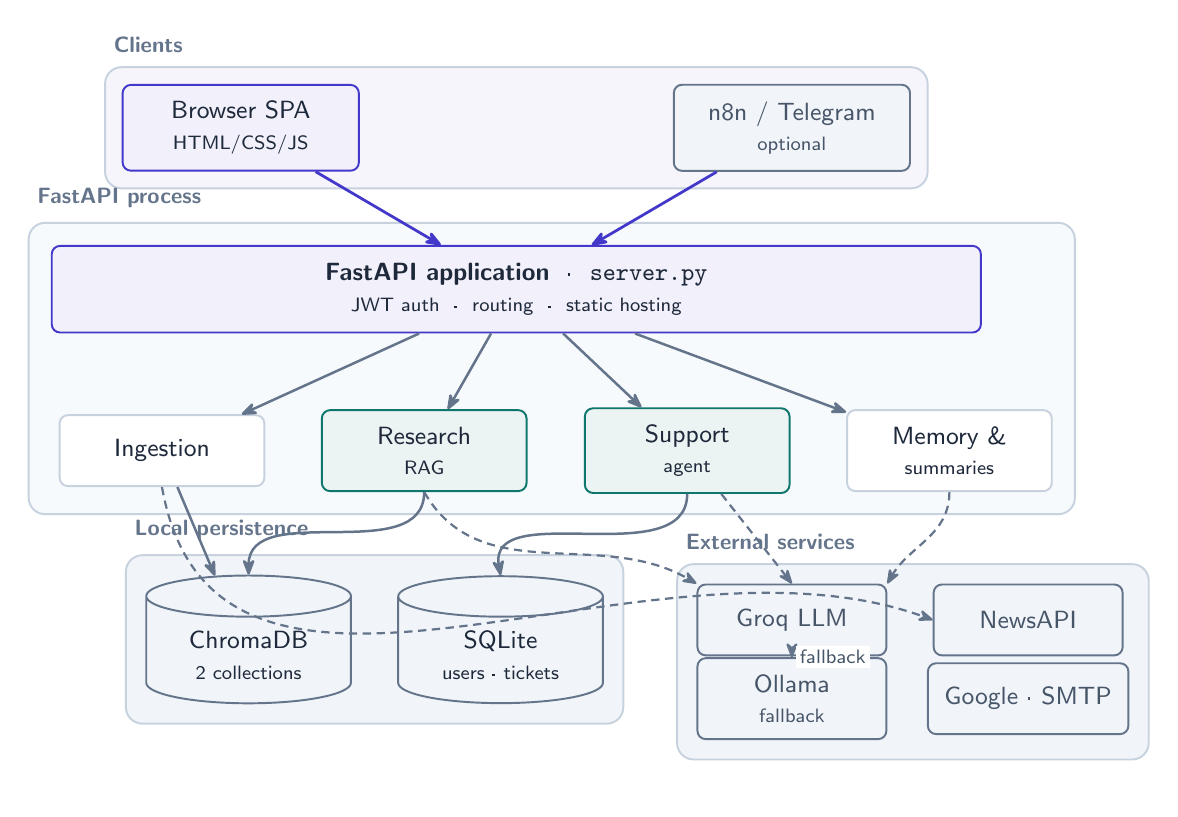
\begin{tikzpicture}[x=1cm,y=1cm]
  % ---- Clients ----
  \node[accentbox, minimum width=30mm] (web) at (2.6,0) {Browser SPA\\{\scriptsize HTML/CSS/JS}};
  \node[ext,       minimum width=30mm] (n8n) at (9.6,0) {n8n / Telegram\\{\scriptsize optional}};

  % ---- API ----
  \node[accentbox, minimum width=118mm, minimum height=11mm] (api) at (6.1,-2.05)
     {\textbf{FastAPI application}\ \ ·\ \ \code{server.py}\\{\scriptsize JWT auth\ \ ·\ \ routing\ \ ·\ \ static hosting}};

  % ---- Capabilities ----
  \node[base,     minimum width=26mm] (ing) at (1.6,-4.1) {Ingestion};
  \node[tealbox,  minimum width=26mm] (res) at (4.93,-4.1) {Research\\{\scriptsize RAG}};
  \node[tealbox,  minimum width=26mm] (sup) at (8.27,-4.1) {Support\\{\scriptsize agent}};
  \node[base,     minimum width=26mm] (mem) at (11.6,-4.1) {Memory \&\\{\scriptsize summaries}};

  % ---- Persistence ----
  \node[store, minimum width=26mm] (chroma) at (2.7,-6.7) {ChromaDB\\{\scriptsize 2 collections}};
  \node[store, minimum width=26mm] (sqlite) at (5.9,-6.7) {SQLite\\{\scriptsize users · tickets}};

  % ---- External ----
  \node[ext, minimum width=24mm] (groq)  at (9.6,-6.25) {Groq LLM};
  \node[ext, minimum width=24mm] (news)  at (12.6,-6.25) {NewsAPI};
  \node[ext, minimum width=24mm] (ollama)at (9.6,-7.25) {Ollama\\{\scriptsize fallback}};
  \node[ext, minimum width=24mm] (oauth) at (12.6,-7.25) {Google · SMTP};

  % ---- Backdrops ----
  \begin{scope}[on background layer]
    \node[group, fill=accent!5, fit=(web)(n8n), inner sep=6pt] (gclients) {};
    \node[group, fit=(api)(ing)(mem), inner sep=8pt] (gapp) {};
    \node[group, fill=mist, fit=(chroma)(sqlite), inner xsep=7pt, inner ysep=7pt] (gstore) {};
    \node[group, fill=mist, fit=(groq)(news)(ollama)(oauth), inner sep=7pt] (gext) {};
  \end{scope}
  \node[grouplabel, anchor=south west, yshift=1.5pt] at (gclients.north west) {Clients};
  \node[grouplabel, anchor=south west, yshift=1.5pt] at (gapp.north west) {FastAPI process};
  \node[grouplabel, anchor=south west, yshift=1.5pt] at (gstore.north west) {Local persistence};
  \node[grouplabel, anchor=south west, yshift=1.5pt] at (gext.north west) {External services};

  % ---- Edges ----
  \draw[flowa] (web) -- (api);
  \draw[flowa] (n8n) -- (api);
  \draw[flow] (api) -- (ing);
  \draw[flow] (api) -- (res);
  \draw[flow] (api) -- (sup);
  \draw[flow] (api) -- (mem);

  \draw[flow] (ing) -- (chroma);
  \draw[flow] (res.south) to[out=-90,in=90] (chroma.north);
  \draw[flow] (sup.south) to[out=-90,in=100] (sqlite.north);

  \draw[dashflow] (res.south) to[out=-60,in=150] (groq.north west);
  \draw[dashflow] (sup) -- (groq.north);
  \draw[dashflow] (mem) to[out=-90,in=60] (groq.north east);
  \draw[dashflow] (ing.south) to[out=-80,in=160] (news.west);
  \draw[dashflow] (groq) -- (ollama) node[tag,midway,right=1pt]{fallback};
\end{tikzpicture}

\caption{High-level runtime. Clients reach a single FastAPI application that fans
out to four internal capabilities backed by local persistence and external APIs.}
\end{figure}

\begin{note}
\textbf{Startup contract.} If \code{GROQ\_API\_KEY} is present, the app builds the
vector engine, bootstraps the support knowledge base, and wires up the research
flow. If it is absent, the components stay uninitialized and the routes that need
them return \code{503} rather than crashing --- the server still starts and serves
the frontend.
\end{note}

% ============================================================
\section{The dual knowledge-base design}
\label{sec:dualkb}

Embeddings come from HuggingFace \code{all-MiniLM-L6-v2} (384-dimension,
normalized), shared by both stores. Chroma then keeps two kinds of collection that
never mix:

\begin{figure}[H]
\centering
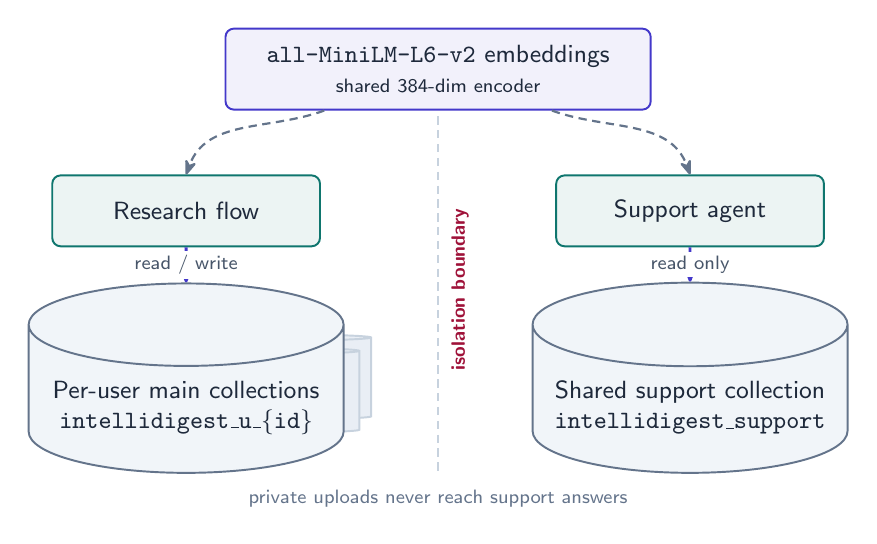
\begin{tikzpicture}[x=1cm,y=1cm]
  % shared embeddings
  \node[accentbox, minimum width=54mm] (emb) at (5,1.6)
     {\code{all-MiniLM-L6-v2} embeddings\\{\scriptsize shared 384-dim encoder}};

  % surfaces
  \node[tealbox, minimum width=34mm] (res) at (1.8,-0.2) {Research flow};
  \node[tealbox, minimum width=34mm] (sup) at (8.2,-0.2) {Support agent};

  % collections
  \node[store, minimum width=40mm] (usc) at (1.8,-2.7)
     {Per-user main collections\\{\scriptsize \code{intellidigest\_u\_\{id\}}}};
  % stacked hint
  \begin{scope}[on background layer]
    \node[store, minimum width=40mm, draw=line, fill=mist2] at (2.15,-2.35) {};
    \node[store, minimum width=40mm, draw=line, fill=mist2] at (2.0,-2.52) {};
  \end{scope}

  \node[store, minimum width=40mm] (spc) at (8.2,-2.7)
     {Shared support collection\\{\scriptsize \code{intellidigest\_support}}};

  % edges
  \draw[dashflow] (emb) to[out=200,in=70] (res.north);
  \draw[dashflow] (emb) to[out=-20,in=110] (sup.north);
  \draw[flowa] (res) -- (usc) node[tag,midway]{read / write};
  \draw[flowa] (sup) -- (spc) node[tag,midway]{read only};

  % isolation boundary
  \draw[line, line width=1pt, densely dashed] (5,1.0) -- (5,-3.5);
  \node[rotate=90, font=\sffamily\scriptsize\bfseries, text=rose] at (5.28,-1.2)
     {isolation boundary};
  \node[font=\sffamily\scriptsize, text=slate, align=center] at (5,-3.85)
     {private uploads never reach support answers};
\end{tikzpicture}

\caption{Retrieval isolation. The research flow only ever reads a user's own
collection; the support agent only ever reads the shared, curated support
collection.}
\end{figure}

\begin{itemize}
  \item \code{intellidigest\_u\_\{id\}} --- one \kw{main} collection per authenticated user, holding their uploads, ingested news, and any n8n-pushed content. Named from a stable hash of the user id.
  \item \code{intellidigest\_support} --- a single \kw{shared} collection seeded from curated \code{support/kb/*.md} files, bootstrapped on first run if empty.
\end{itemize}

\noindent The payoff is a hard guarantee: a user's private documents can never
surface inside a scripted support answer, and one user's uploads are never visible
to another. The isolation is structural, enforced by which collection each code
path is allowed to open --- not by a filter that could be forgotten.

% ============================================================
\section{Data flows}
\label{sec:flows}

\subsection{Ingestion into the main knowledge base}
Everything that adds text to a user's collection follows the same path:
\emph{raw content $\rightarrow$ chunk $\rightarrow$ embed $\rightarrow$ Chroma}.
Uploads are parsed per format and semantically chunked on sentence boundaries; news
articles are fetched from NewsAPI and de-duplicated by URL before embedding.

\begin{figure}[H]
\centering
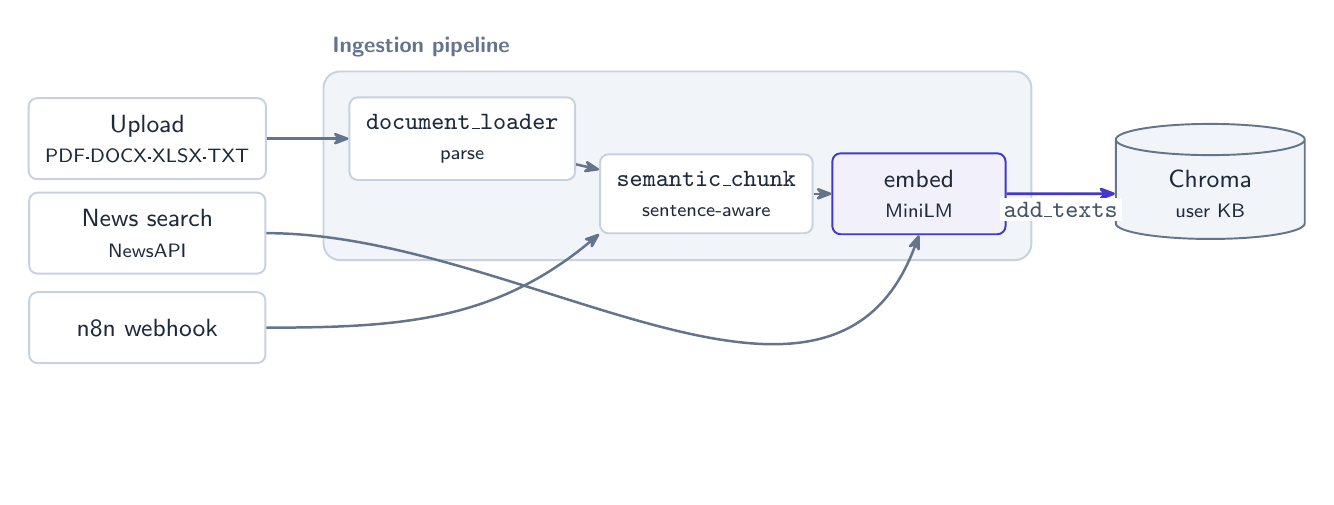
\begin{tikzpicture}[x=1cm,y=1cm]
  % sources
  \node[base, minimum width=30mm] (up) at (0,1.2) {Upload\\{\scriptsize PDF·DOCX·XLSX·TXT}};
  \node[base, minimum width=30mm] (nw) at (0,0)   {News search\\{\scriptsize NewsAPI}};
  \node[base, minimum width=30mm] (wh) at (0,-1.2){n8n webhook};

  % pipeline
  \node[base,      minimum width=26mm] (load)  at (4.0,1.2) {\code{document\_loader}\\{\scriptsize parse}};
  \node[base,      minimum width=26mm] (chunk) at (7.1,0.5) {\code{semantic\_chunk}\\{\scriptsize sentence-aware}};
  \node[accentbox, minimum width=22mm] (embed) at (9.8,0.5) {embed\\{\scriptsize MiniLM}};
  \node[store,     minimum width=24mm] (kb)    at (13.5,0.5) {Chroma\\{\scriptsize user KB}};

  \begin{scope}[on background layer]
    \node[group, fill=mist, fit=(load)(chunk)(embed), inner sep=9pt] (gp) {};
  \end{scope}
  \node[grouplabel, anchor=south west, yshift=1.5pt] at (gp.north west) {Ingestion pipeline};

  % edges
  \draw[flow] (up) -- (load);
  \draw[flow] (load) -- (chunk);
  \draw[flow] (wh.east) to[out=0,in=-140] (chunk.south west);
  \draw[flow] (nw.east) to[out=0,in=-110] (embed.south);
  \draw[flow] (chunk) -- (embed);
  \draw[flowa] (embed) -- (kb) node[tag,midway,below=1pt]{\code{add\_texts}};
\end{tikzpicture}

\caption{Three sources converge on one embedding-and-store path, all scoped to the
authenticated user's collection.}
\end{figure}

\subsection{Research chat}
The research surface retrieves the top-$k$ chunks from the user's collection, builds
a prompt from the persona, the retrieved context, and the compressed chat history,
then calls the LLM stack. The answer is parsed for inline follow-up suggestions and
returned with its sources; the exchange is folded back into memory.

\begin{figure}[H]
\centering
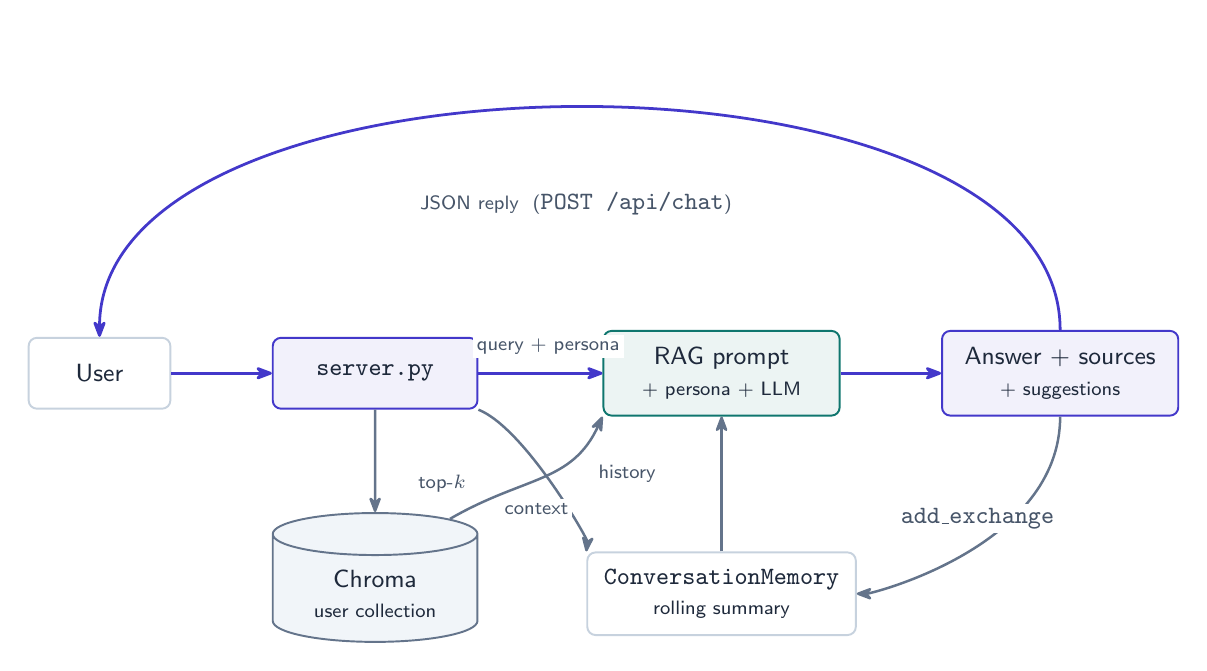
\begin{tikzpicture}[x=1cm,y=1cm]
  \node[base,      minimum width=18mm] (user) at (0,0)    {User};
  \node[accentbox, minimum width=26mm] (api)  at (3.5,0)  {\code{server.py}};
  \node[tealbox,   minimum width=30mm] (gen)  at (7.9,0)  {RAG prompt\\{\scriptsize + persona + LLM}};
  \node[accentbox, minimum width=30mm] (ans)  at (12.2,0) {Answer + sources\\{\scriptsize + suggestions}};

  \node[store, minimum width=26mm] (vs)  at (3.5,-2.8) {Chroma\\{\scriptsize user collection}};
  \node[base,  minimum width=32mm] (mem) at (7.9,-2.8) {\code{ConversationMemory}\\{\scriptsize rolling summary}};

  % main horizontal path
  \draw[flowa] (user) -- (api);
  \draw[flowa] (api) -- (gen);
  \draw[flowa] (gen) -- (ans);

  % retrieval + memory
  \draw[flow] (api) -- (vs);
  \draw[flow] (api.south east) .. controls (5.4,-0.7) and (6.2,-2.1) .. (mem.north west);
  \draw[flow] (vs.north east) .. controls (5.4,-1.3) and (6.0,-1.4) .. (gen.south west);
  \draw[flow] (mem.north) -- (gen.south);

  % write-back (stays on the right)
  \draw[flow] (ans.south) .. controls (12.2,-2.2) and (9.8,-2.8) .. (mem.east);

  % top return arc
  \draw[flowa] (ans.north) to[out=90,in=90,looseness=0.8] (user.north);

  % ---- fixed-position labels ----
  \node[tag] at (6.05,2.15) {JSON reply\ \ (\code{POST /api/chat})};
  \node[tag] at (5.7,0.34)  {query + persona};
  \node[tag] at (4.35,-1.4) {top-$k$};
  \node[tag] at (5.55,-1.72){context};
  \node[tag] at (6.7,-1.28) {history};
  \node[tag] at (11.15,-1.85){\code{add\_exchange}};
\end{tikzpicture}

\caption{Request path for \code{POST /api/chat}. Retrieval and memory both feed the
single generation call; the reply updates memory before it returns.}
\end{figure}

\begin{note}
\textbf{Memory compression.} \code{ConversationMemory} keeps recent turns verbatim
and, once history grows past a threshold, compresses older exchanges into a running
summary with the LLM. Long conversations stay inside the context window without
losing their thread.
\end{note}

\subsection{Support agent and ticketing}
The support surface is a genuine LangChain \code{AgentExecutor} built with
\code{create\_tool\_calling\_agent}. The model decides which tools to call:

\begin{figure}[H]
\centering
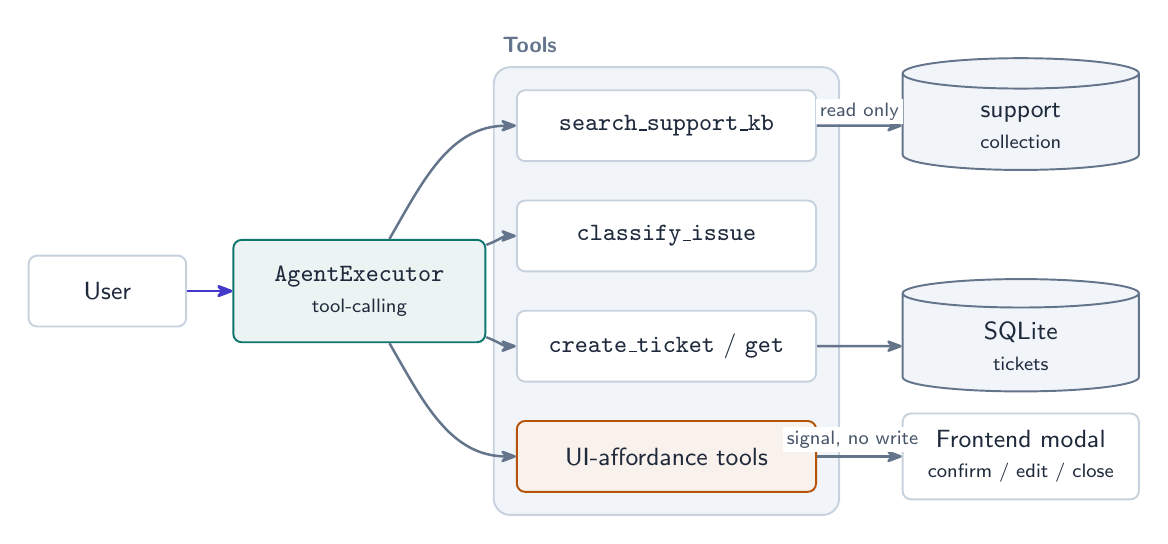
\begin{tikzpicture}[x=1cm,y=1cm]
  \node[base,    minimum width=20mm] (user)  at (0,0) {User};
  \node[tealbox, minimum width=32mm, minimum height=13mm] (agent) at (3.2,0)
     {\code{AgentExecutor}\\{\scriptsize tool-calling}};

  % tools
  \node[base, minimum width=38mm] (t1) at (7.1,2.1)  {\code{search\_support\_kb}};
  \node[base, minimum width=38mm] (t2) at (7.1,0.7)  {\code{classify\_issue}};
  \node[base, minimum width=38mm] (t3) at (7.1,-0.7) {\code{create\_ticket} / \code{get}};
  \node[amberbox, minimum width=38mm] (t4) at (7.1,-2.1) {UI-affordance tools};

  % targets
  \node[store, minimum width=30mm] (skb) at (11.6,2.1)  {support\\{\scriptsize collection}};
  \node[store, minimum width=30mm] (db)  at (11.6,-0.7) {SQLite\\{\scriptsize tickets}};
  \node[base,  minimum width=30mm] (fe)  at (11.6,-2.1) {Frontend modal\\{\scriptsize confirm / edit / close}};

  \begin{scope}[on background layer]
    \node[group, fill=mist, fit=(t1)(t2)(t3)(t4), inner sep=8pt] (gt) {};
  \end{scope}
  \node[grouplabel, anchor=south west, yshift=1.5pt] at (gt.north west) {Tools};

  \draw[flowa] (user) -- (agent);
  \draw[flow] (agent) to[out=60,in=180]  (t1);
  \draw[flow] (agent) to[out=20,in=180]  (t2);
  \draw[flow] (agent) to[out=-20,in=180] (t3);
  \draw[flow] (agent) to[out=-60,in=180] (t4);

  \draw[flow] (t1) -- (skb) node[tag,midway,above]{read only};
  \draw[flow] (t3) -- (db);
  \draw[flow] (t4) -- (fe) node[tag,pos=0.42,above=1pt]{\scriptsize signal, no write};
\end{tikzpicture}

\caption{The support agent reasons over four tool families. Knowledge search is
restricted to the support collection; UI-affordance tools only signal the frontend,
they never mutate the database.}
\end{figure}

\begin{itemize}
  \item \code{search\_support\_knowledge\_base} --- retrieves from the support collection \emph{only}.
  \item \code{classify\_issue} --- assigns a category and priority.
  \item \code{create\_ticket} / \code{get\_ticket} --- read and write SQLite ticket rows.
  \item \textbf{UI-affordance tools} --- \code{show\_confirm\_close}, \code{show\_edit\_ticket}, and friends emit a signal the frontend turns into a confirmation modal. They perform \emph{no} database writes.
\end{itemize}

\noindent Destructive changes (closing or editing a ticket) therefore go through an
explicit REST call after the user confirms in the UI --- the model can propose a
mutation, but it cannot silently commit one.

% ============================================================
\section{LLM strategy and resilience}
\label{sec:llm}

A single factory (\code{chains/llm\_factory.py}) builds every chat model in the
system. It supports a bring-your-own-key choice of provider (Groq, OpenAI, or
Gemini) and always wraps the primary model with a local Ollama fallback via
LangChain's \code{RunnableWithFallbacks}. Rate limits, timeouts, connection errors,
and server errors are all caught and retried against the local model, so a provider
outage degrades quality instead of breaking the request.

\begin{figure}[H]
\centering
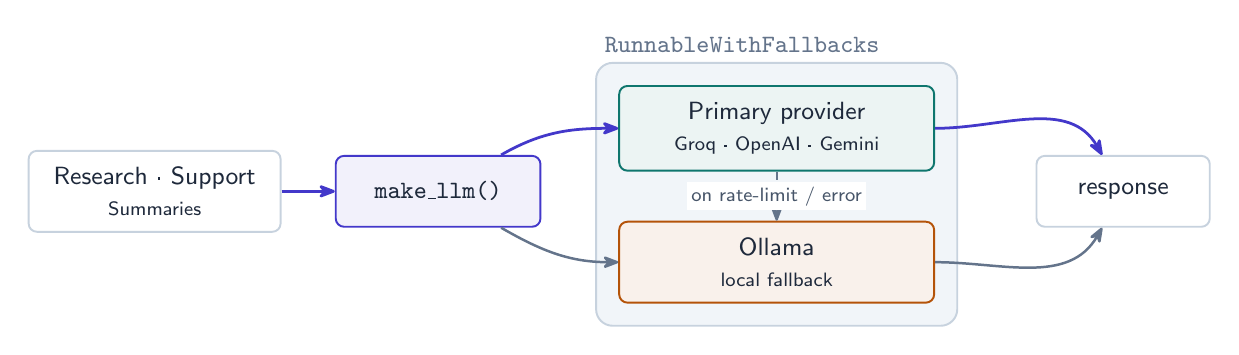
\begin{tikzpicture}[x=1cm,y=1cm]
  \node[base,      minimum width=32mm] (cons) at (0,0) {Research · Support\\{\scriptsize Summaries}};
  \node[accentbox, minimum width=26mm] (fac)  at (3.6,0) {\code{make\_llm()}};
  \node[tealbox,   minimum width=40mm] (prim) at (7.9,0.8) {Primary provider\\{\scriptsize Groq · OpenAI · Gemini}};
  \node[amberbox,  minimum width=40mm] (olla) at (7.9,-0.9) {Ollama\\{\scriptsize local fallback}};
  \node[base,      minimum width=22mm] (out)  at (12.3,0) {response};

  \begin{scope}[on background layer]
    \node[group, fill=mist, fit=(prim)(olla), inner sep=8pt] (gw) {};
  \end{scope}
  \node[grouplabel, anchor=south west] at (gw.north west) {\code{RunnableWithFallbacks}};

  \draw[flowa] (cons) -- (fac);
  \draw[flowa] (fac) to[out=30,in=180]  (prim);
  \draw[flow]  (fac) to[out=-30,in=180] (olla);
  \draw[flowa] (prim) to[out=0,in=120] (out);
  \draw[dashflow]  (prim) -- (olla) node[tag,midway]{on rate-limit / error};
  \draw[flow]  (olla) to[out=0,in=-120] (out);
\end{tikzpicture}

\caption{Every chain and agent in the system is constructed through one factory, so
the fallback behavior is uniform across research, support, and summarization.}
\end{figure}

% ============================================================
\section{Interface surface}
\label{sec:api}

The frontend is a single hand-written HTML/CSS/JS page --- no framework, no build
step --- talking to a REST API. The table below groups the most important
endpoints; every data route requires a JWT bearer token.

\begin{table}[H]
\small
\setlength{\tabcolsep}{7pt}\renewcommand{\arraystretch}{1.25}
\begin{tabularx}{\linewidth}{@{}l l L@{}}
\toprule
\sffamily\bfseries Area & \sffamily\bfseries Endpoint & \sffamily\bfseries Purpose \\
\midrule
Auth     & \code{POST /api/auth/register} & Email/password sign-up, returns JWT \\
Auth     & \code{POST /api/auth/login}    & Login, returns JWT \\
Auth     & \code{GET\ \ /api/auth/google}  & Begin Google OAuth \\
Ingest   & \code{POST /api/upload}        & Parse, chunk, and embed a document \\
Ingest   & \code{POST /api/news/search}   & Fetch and ingest news articles \\
Research & \code{POST /api/chat}          & Grounded, persona-aware answer + sources \\
Research & \code{GET\ \ /api/search}       & Semantic search over the main collection \\
Research & \code{POST /api/summarize}     & Brief (stuff) or detailed (map-reduce) summary \\
Support  & \code{POST /api/support/chat}  & Tool-calling support agent \\
Support  & \code{GET\ \ /api/tickets}      & List the user's tickets \\
Support  & \code{POST /api/tickets/\{id\}/close} & Close a ticket after confirmation \\
Ops      & \code{GET\ \ /health}           & Liveness probe (does not block on model load) \\
\bottomrule
\end{tabularx}
\caption{Representative REST surface. Per-user isolation is enforced server-side
from the authenticated identity in the token.}
\end{table}

% ============================================================
\section{Technology stack}
\label{sec:stack}

\begin{table}[H]
\small
\setlength{\tabcolsep}{7pt}\renewcommand{\arraystretch}{1.25}
\begin{tabularx}{\linewidth}{@{}l L@{}}
\toprule
\sffamily\bfseries Layer & \sffamily\bfseries Choice and rationale \\
\midrule
Orchestration & \textbf{LangChain} --- LCEL chains, \code{AgentExecutor}, prompt templates, memory \\
Primary LLM   & \textbf{Groq} (Llama 3.3 70B) --- fast inference for chat, RAG, and summaries \\
Fallback LLM  & \textbf{Ollama} (local) --- keeps the app answering when the provider fails \\
Embeddings    & \textbf{HuggingFace} \code{all-MiniLM-L6-v2} --- compact, CPU-friendly, normalized \\
Vector store  & \textbf{ChromaDB} --- persistent, per-user main + shared support collections \\
API           & \textbf{FastAPI} --- async routes, dependency-injected auth, static hosting \\
Persistence   & \textbf{SQLite} --- users and support tickets under a configurable data root \\
Frontend      & \textbf{Vanilla HTML/CSS/JS} --- a design-tokened SPA with no build step \\
Automation    & \textbf{n8n} (optional) --- webhook bridge for Telegram delivery \\
\bottomrule
\end{tabularx}
\caption{Deliberately lean stack: one process, local persistence, and a single
orchestration library across every AI surface.}
\end{table}

\subsection{Engineering notes}
\begin{itemize}
  \item \textbf{Deferred heavy imports.} Embeddings and LangChain load in a background thread so uvicorn binds before the model is ready --- important for container health checks.
  \item \textbf{Per-user collection naming.} A user id is normalized to a stable 32-character suffix (hashed when needed) so a collection maps deterministically to an account.
  \item \textbf{News de-duplication.} Articles are checked against existing URLs in the collection before embedding, preventing duplicate chunks on repeated searches.
  \item \textbf{Confirmation-gated mutations.} The support agent surfaces intent to the UI; the actual write happens over REST only after the user confirms.
  \item \textbf{Tested auth core.} The authentication and token paths are covered by an automated \code{pytest} suite.
\end{itemize}

\vspace{2mm}
\begin{note}
\textbf{Summary.} One FastAPI process, two isolated vector collections, one LLM
factory with a built-in safety net, and a clean split between a grounded research
surface and a tool-driven support surface. The architecture optimizes for privacy,
resilience, and a demo that keeps working when the network does not.
\end{note}

\end{document}
